\documentclass{article}
\usepackage{graphicx}
\usepackage[T2A]{fontenc}
\usepackage[utf8]{inputenc}
\usepackage[russian]{babel}
\usepackage{alltt}
\usepackage{amsmath}
\usepackage{amsfonts}
\usepackage{indentfirst}
\usepackage{layout}
\usepackage{hyperref}
\usepackage{geometry}
\usepackage{pdfpages}
\usepackage{svg}
\geometry{
	a4paper,
	top=25mm,
	right=15mm,
	bottom=25mm,
	left=30mm
}
\makeatletter
\paragraph{\@startsection{paragraph}{4}{\z@}%
% display heading, like subsubsection
                                     {-3.25ex\@plus -1ex \@minus -.2ex}%
                                     {1.5ex \@plus .2ex}%
                                     {\normalfont\normalsize\bfseries}}
 \setcounter{secnumdepth}{4}
\makeatother
\title{non-linear equations}
\author{Иван Золин, Святослав Гвоздев, Евгений Хламкин}
\date{September 2022}
\thispagestyle{empty}
\begin{document}

	\large
	\begin{center}

		Санкт-Петербургский политехнический университет\\
		Высшая школа прикладной математики и вычислительной физики, ФизМех

		~\\
		~\\
		~\\
		~\\
		Направление подготовки\\
		«01.03.02 Прикладная математика и информатика»\\
		Специальность «Системное программирование»
		~\\
		~\\
		~\\
		~\\
	Лабораторная работа №1\\
		\textbf{"Решение задачи линейного программирования. Симплекс - Метод. Метод перебора крайних точек"}\\
	дисциплина "Методы оптимизации"\\
	\end{center}
	~\\
	~\\
	~\\
	~\\
	~\\
	~\\
	~\\
	\begin{alltt}
        	Выполнили студенты гр. 5030102/00201		      Гвоздев С.Ю.,
        		                                           Золин И.М.
        		                                           Хламкин Е.В.

        	Преподаватель: 				              	            Родионова Е.А.
	\end{alltt}

	~\\
	~\\
	~\\
	~\\
	~\\
	~\\
	~\\
	~\\
	~\\
	~\\
	~\\
	\begin{center}
		Санкт-Петербург

		~\\
		\textbf{2023}
	\end{center}

	\newpage
	\tableofcontents
	\newpage
	\section{Постановка задачи}
     Поставлена задача линейного программирования, состоящая из 6 переменных, 3 равенств, 2 неравенств $"\leq "$, 1 неравенства $"\geq"$. Также поставлены ограничения на знаки для 3 переменных:
    \begin{equation*}
     \begin{cases}
      -23x_1 + 3x_2 + x_3 - 2x_4 - 3x_5 - 5x_6\le 17
      \\
      -18x_1 + 3x_2 + x_3 - 3x_4 - 3x_5 - 4x_6\le 12
       \\
       13x_1 - 3x_2 - x_3 + 3x_4 + 3x_5 +3x_6\ge -13
       \\
       -8x_1 + 3x_2 + x_3 - 2x_4 - 2x_5 -2x_6 = 23
       \\
       -4x_1 + 2x_2 + x_3 - x_4 - x_5 - x_6 = 20
       \\
       -4x_1 + 2x_2 + 2x_3 - x_4 - x_5 -x_6 = 29
       \\
       x_1, x_2, x_3 \ge 0
     \end{cases}
    \end{equation*}
    Функция цели:
    \begin{equation}
    F(x) =  4x_1 + 6x_2 + 2x_3 + 6x_4 + 5x_5 + 3x_6\longrightarrow min
    \end{equation}
    Необходимо:
    \begin{enumerate}
        \item Решить данную задачу Симплекс - Методом
        \item Решить данную задачу методом перебора крайних точек.
        \item Провести анализ и сравнение полученных результатов. Привести качественный разбор скорости сходимости Симплекс - Метода и метода перебора крайних точек
        \item Построить двойственную задачу к данной
    \end{enumerate}

	\section{Исследование применимости метода}
    Алгоритм \textbf{симплекс-метода} применим к задачам линейного программирования на поиск минимума путем перебора вершин выпуклого многранника в многогранном пространстве.

    Метод является универсальным и применим к любой задаче, работает на задачах в канонической форме при всяких вещественных значениях компонент $ A \in \mathbb{R}_{m\times{n}}, b \in \mathbb{R}_{m}, c \in \mathbb{R}_n $.
	Матрица $A$ должно иметь ранг $m$, что гарантирует наличие хотя бы одного опорного вектора.

    Данная задача соответствует вышеуказанным условиям, так как формировалась изначально с помощью единичной матрицы и положительного вектора $b$, а потом с помощью эквивалентных преобразований (сложение строк и умножение строк на число) приводилась к нетривиальной форме.
	\section{Описание алгоритма}
    \subsection{Алгоритм симплекс метода}
    \subsubsection{Описание}
    \textbf{Input}: задача линейного программирования
			в стандартной форме\\
    \textbf{Output}: вектор $x[N]$, который является оптимальным решением задачи линейного программирования, или сообщение о неразрешимости или неограниченности задачи
    \subsubsection{Блок-схема}
    \begin{center}
         \includesvg[height=0.9\textheight]{graphics/simplex.svg}
    \end{center}
    \subsubsection{Правило Блэнда}
    Правило Блэнда - усовершенстоввание симплекс-метода, направленное на нахождение решения без зацикливания.(Если Симплекс метод не может завершиться более чем за $C^M_{N}$, то он зацикливается) [1]

    Обычно целевая функция действительно уменьшается на каждом шаге, и таким образом после ограниченного числа шагов находится оптимальное решение. Однако есть примеры вырожденных линейных программ, на которых исходный симплексный алгоритм зацикливается вечно.

    \textbf{Алгоритм}
    \begin{enumerate}
        \item Выбираем небазисный столбец с наименьшим номером
        \item Среди всех строк выбираем ту, для которой минимум отношения правой части и коэффициента вводимого столбца в таблице(при условии, что этот коэффицинт больше 0). Если такой минимум достигается на нескольких строках, выбираем ту, которая соотвествует столбцу с наименьшим индексом.
    \end{enumerate}

    \textbf{Пример}\\
    \begin{enumerate}
        \item Целевая функция: $c = 10\textcolor{red}{x_1} - 57x_2 - 9x_3 - 24x_4$\\
    $\textcolor{blue}{x_5} = -0.5x_1 + 5.5x_2 + 2.5x_3 - 9x_4$\\
    $x_6= -0.5x_1 + 1.5x_2 + 0.5x_3 - x_4$\\
    $x_7 = 1 - x_1$\\
    (0, 0, 0, 0, [0], [0],[1]) $x_1$-вх, $x_5$-вых

    \item Целевая функция: $c = 53\textcolor{red}{x_2} + 41x_3 - 204x_4 - 20x_5$\\
    $x_1 = 11x_2 + 5x_3 - 18x_4 - 2x_5$\\
    $\textcolor{blue}{x_6} = -4x_2 - 2x_3 + 8x_4 + x_5$\\
    $x_7 = 1 - 11x_2 - 5x_3 + 18x_4 + 2x_5$\\
    ([0], 0, 0, 0, 0, [0],[1]) $x_2$-вх, $x_6$-вых

    \item Целевая функция: $c = 14.5\textcolor{red}{x_3} - 98x_4 - 6.75x_5 - 13.25x_6$\\
    $\textcolor{blue}{x_1} = -0.5x_3 + 4x_4 + 0.75x_5 - 2.75x_6$\\
    $x_2 = -0.5x_3 + 2x_4 + 0.25x_5 - 0.25x_6$\\
    $x_7 = 1 + 0.5x_3 - 4x_4 - 0.75x_5 - 13.25x_6$\\
    ([0], [0], 0, 0, 0, 0,[1]) $x_3$-вх, $x_1$-вых

    \item Целевая функция: $c = -29x_1 + 18\textcolor{red}{x_4} + 15x_5 - 93x_6$\\
    $x_3 = -2x_1 + 8x_4 + 1.5x_5 - 5.5x_6$\\
    $\textcolor{blue}{x_2} = x_1 - 2x_4 - 0.5x_5 + 2.5x_6$\\
    $x_7 = 1 - x_1$\\
    (0, [0], [0], 0, 0, 0,[1]) $x_4$-вх, $x_2$-вых

    \item Целевая функция: $c = -20x_1 - 9x_2 + 10.5\textcolor{red}{x_5} - 70.5x_6$\\
    $\textcolor{blue}{x_3} = 2x_1 - 4x_2  - 0.5x_5 + 4.5x_6$\\
    $x_4 = 0.5x_1 - 0.5x_2 - 0.25x_5 + 1.25x_6$\\
    $x_7 = 1 - x_1$\\
    (0, 0, [0], [0], 0, 0,[1]) $x_5$-вх, $x_3$-вых

    \item Следующая поворотная точка позволяет нам выйти из цикла (цикл возникает, если $x_6$ выбирается для входа).

    Целевая функция: $c = 22\textcolor{red}{x_1} - 93x_2 - 21x_3 + 24x_6$\\
    $x_5 = 4x_1 - 8x_2 - 2x_3 + 9x_6$\\
    $\textcolor{blue}{x_4} = -0.5x_1 + 1.5x_2 + 0.5x_3 - x_6$\\
    $x_7 = 1 - x_1$\\
    (0, 0, 0, [0], [0], 0,[1]) $x_1$-вх, $x_4$-вых

    \item Целевая функция: $c = -27x_2 + \textcolor{red}{x_3} - 44x_4 - 20x_6$\\
    $x_5 = 4x_2 + 2x_3 - 8x_4 + x_6$\\
    $x_1 = 3x_2 + x_3 - 2x_4 - 2x_6$\\
    $\textcolor{blue}{x_7} = 1 - 3x_2 - x_3 + 2x_4 + 2x_6$\\
    ([0], 0, 0, 0, [0], 0,[1]) $x_3$-вх, $x_7$-вых

    \item Целевая функция: $c = 1 - 30x_2-42x_4-18x_6-x_7$\\
    $x_5 = 2 - 2x_2 - 4x_4 +5x_6 - 2x_7$\\
    $x_1 = 1 - x_7$\\
    $x_3 = 1 - 3x_2 + 2x_4 + 2x_6 - x_7$\\
    ([1], 0, [1], 0, [2], 0, 0)
    \end{enumerate}
    Целевая функция имеет максимум = 1, достигаемый в точке (1, 0, 1, 0, 2, 0, 0)

    Заметим, что в вышеописанном процессе решения участвуют только 8 из $C^3_7$= 35

    \subsection{Алгоритм перевода из общей в каноническую форму}
	\textbf{Input}: система уравнений A[M,N] в общей форме\\
    \textbf{Output}: система уравнений A[M,N] в канонической форме
	\begin{enumerate}
		\item Проверяем знаки в системе
		\item Если <<$\le$>>, то к левой части добавляем $w[i]$, если <<$\ge$>>, то из левой части вычитаем $w[i]$, $w[i]\ge0$.
		\item Знаки неравенства в системе заменяем на равенство.
		\item Производим замену переменных: \\если $x[i]\le0$, то $x'[i]=-x[i]\ge0$; \\если $x[i]$ любого знака, то $x[i]=u[i]-v[i]$, $v[i],u[i] \ge 0$.
	\end{enumerate}

    \subsection{Алгоритм восстановления решения двойственной задачи по решению прямой}
    Рассмотрим задачу минимума:
    	\begin{equation*}
              min~c^T[N] \cdot x[N]
            \end{equation*}
            \begin{equation}
            S = \{\ x[N]|~ A[M, N] \cdot x[N] = b[M],~x[N] \ge 0 \}\
            \label{one}
        \end{equation}

    В случае задачи максимума, то домножаем целевой вектор на $-1$.

    Для получения двойственной задачи будем использолвать теоремы двойственности.

     Найдя решение прямой задачи(с оптимальным значением целевой функции $F_{max}$ и оптимальным планом $x = x_1, x_2,..., x_n$), подставив в систему ограничений, проверим:

     Если
     \begin{enumerate}
         \item i-ое неравенство не является равенством ($a_{1i}x_1 + a_{2i}x_2 + ... + a_{mi}x_n \neq c_i$), то $y_i = 0$
         \item $x_k \neq 0$, то k-ая строка системы ограничений является равенством:
         $a_{1k}y_1 + a_{2k}y_2 + ... + a_{mk}y_k = c_k$
     \end{enumerate}
     Система ограничений:

     \begin{equation*}
     \begin{cases}
      a_{11}y_1 + a_{21}y_2 + ... + a_{m1}y_m \ge c_1
      \\
      a_{12}y_1 + a_{22}y_2 + ... + a_{m2}y_m \ge c_2
       \\
       ...
       \\
       a_{1n}y_1 + a_{2n}y_2 + ... + a_{mn}y_m \ge c_n
       \\
       y_1 \ge 0, y_2 \ge 0, ..., y_m \ge 0
       \\
       x_1, x_2  \ge 0
     \end{cases}
    \end{equation*}

    Составим все строки ограничений, для которых $x_k \neq 0$, полуичм систему уравнений, из которых можно найти ненулевые значения переменных y.

    По 1-ой теореме двойственности: минимальное значение целевой функции $z_{min} = F_{max} \Rightarrow$ для получения решения двойственной задачи достаточно решить полученную систему линейных уравнений.\\

    Исходная задача, переведенная в двойственную форму:
\begin{equation*}
    \begin{cases}
      -23y_1 + -18y_2 + 13y_3 - 8y_4 - 4y_5 - 4y_6\leq 4
      \\
      3y_1 + 3y_2 - 3y_3 + 3y_4 + 2y_5 + 2y_6\leq 6
       \\
       y_1 + y_2 + 1y_3 - y_4 + y_5 +2y_6 = 2
       \\
       -2y_1 - 3y_2 + 3y_3 - 2y_4 - y_5 - y_6 = 6
       \\
       -3y_1 - 3y_2 + 3y_3 - 2y_4 - y_5 - y_6 = 5
       \\
       -5y_1 - 4y_2 + 3y_3 - 2y_4 - y_5 -y_6 = 3
       \\
       y_1, y_2 \geq 0, y_3 \leq 0
     \end{cases}
 \end{equation*}

 \begin{equation}\label{eq:goal}
    F(y) =  17y_1 + 12y_2 - 13y_3 + 23y_4 + 20y_5 + 29y_6\longrightarrow max
 \end{equation}

    \subsection{Алгоритм перебора крайних точек}
    Оптимальный вектор в алгоритме перебора крайних точек является угловой точкой ОДР(области допустимых решений). Если же имеется множество решений, то среди них найдутся угловые точки.

    Находя угловые точки - вычисляем в них значяения целевой функции. Далее определяем наименьшее/наибольшее значение функции.

    \textbf{Input}:
    \begin{enumerate}
        \item A[M,N] - матрица коэффициентов задачи в каноничесокой форме
        \item b[M] - вектор свободных коэффициентов задачи
        \item c[N] - вектор коэффициентов функции цели задачи
    \end{enumerate}

    \textbf{Output}: опорный вектор x[N], минимизирующий целевую функцию

    Алгоритм:
    \begin{enumerate}
        \item Генерирование квадратных мтриц, выделямых из A[M,N], где M < N: их количество $C^M_N$
        \item Проверка для каждой матрицы отличие определителя от нуля. Далее, если проверка пройдена, находим решение системы: $A[M, N_k]x[N_k] = b[M]$
        \item Проверка на положительность компонент решения. Если проверка пройдена, то дополняем $x[N]$ нулевыми значениями соответсвующих компонент и получаем крайнюю точку.
        \item Находим значение функции цели в крайней точке и запоминаем его
        \item Повторяем предыдущие шаги
        \item Сравниваем значения между собой и выбираем то решение, которое соотвествует наименьшему значению функции цели.
    \end{enumerate}

    \subsection{Решение поставленной задачи}
    \begin{center}
         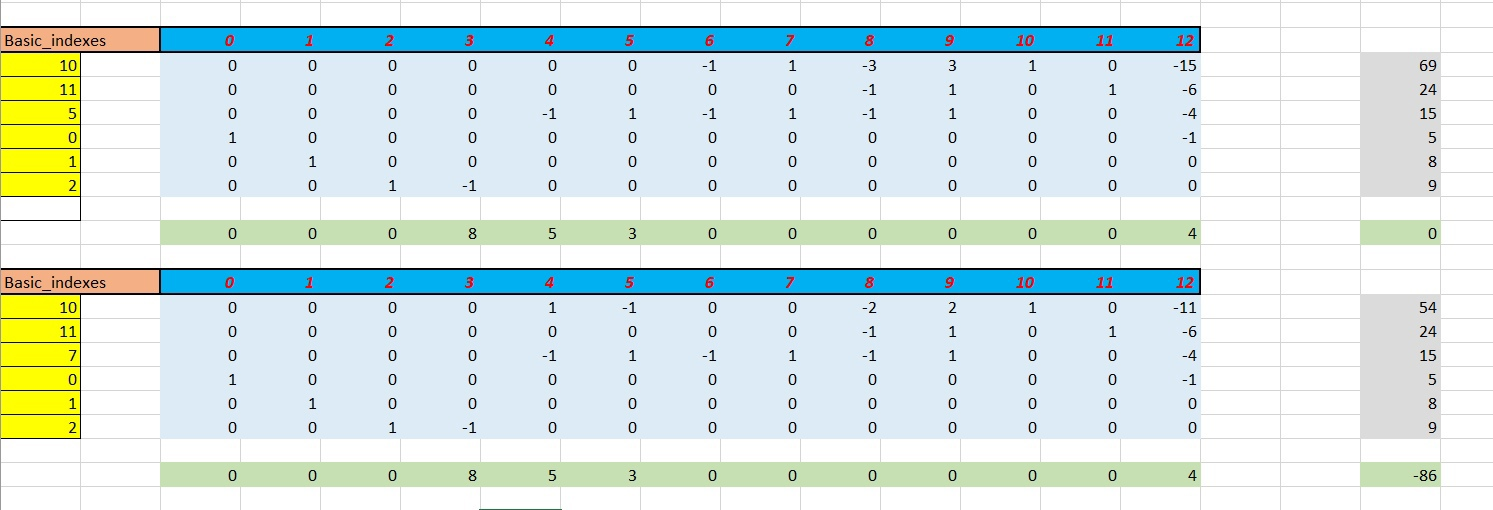
\includegraphics[width=\textwidth]{../graphics/table.jpg}
    \end{center}

    Зднсь первая таблица соответствует процедуре Инициализации Симплекс-Метода (поиск допустимого базиса). Вторая таблица - переход от найденного допустимого базисного решения к новому допустимому базису. Оказывается, что в данном примере Симплекс-Метод решает задачу за одну итерацию.

\newpage
	\section{Обоснование достоверности полученного решения}
    \subsection{Сравнительный анализ}
    \begin{enumerate}
        \item График зависимости времени выполнения метода от размерности матрицы (3,6)
        \begin{center}
         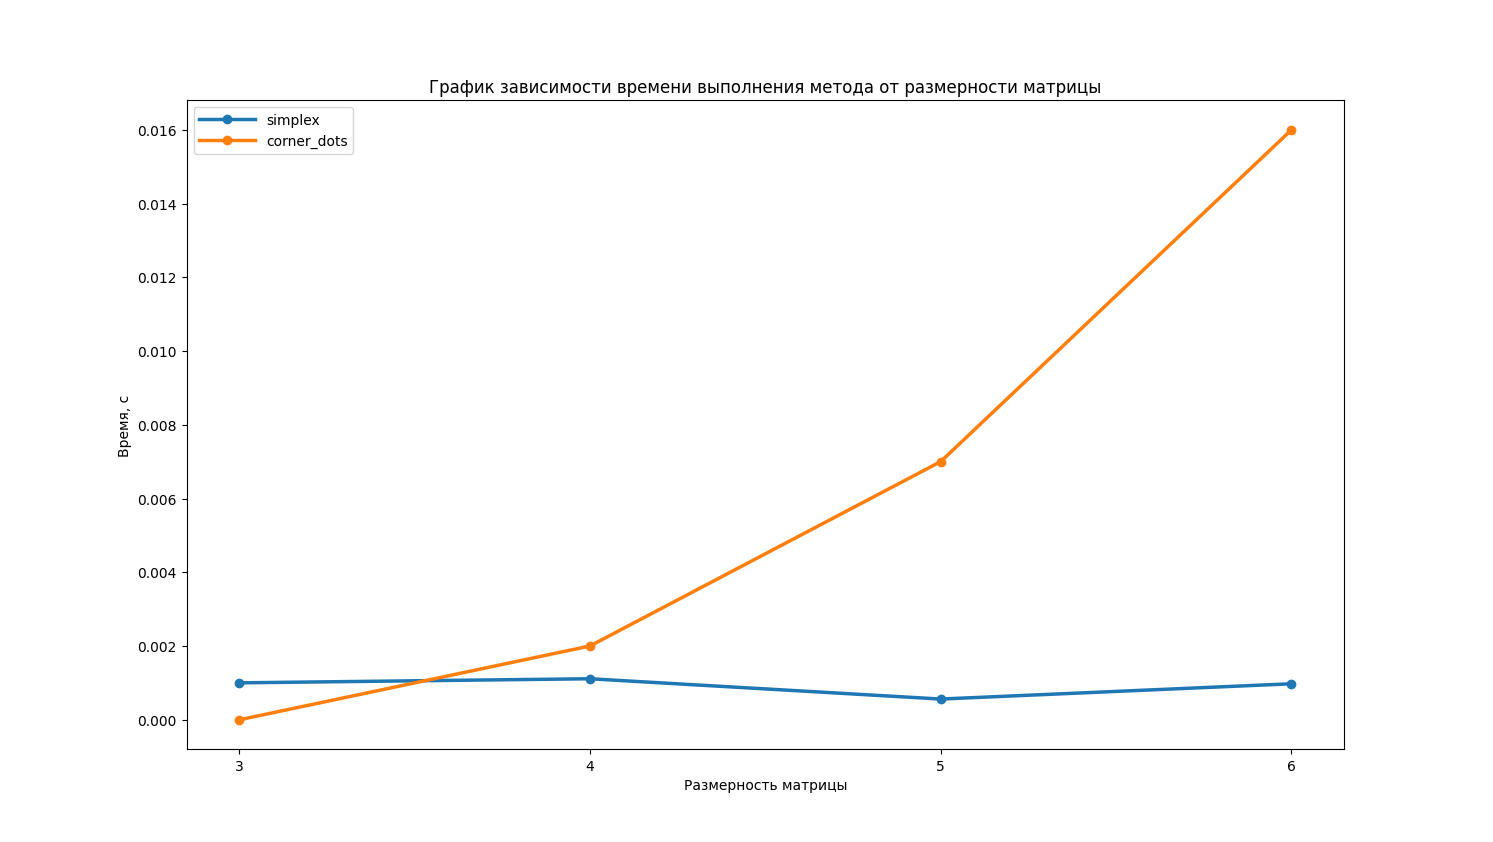
\includegraphics[width=\textwidth]{../graphics/Time_small_rangs_1.png}
        \end{center}
        \item График зависимости времени выполнения метода от размерности матрицы (3,10)
        \begin{center}
         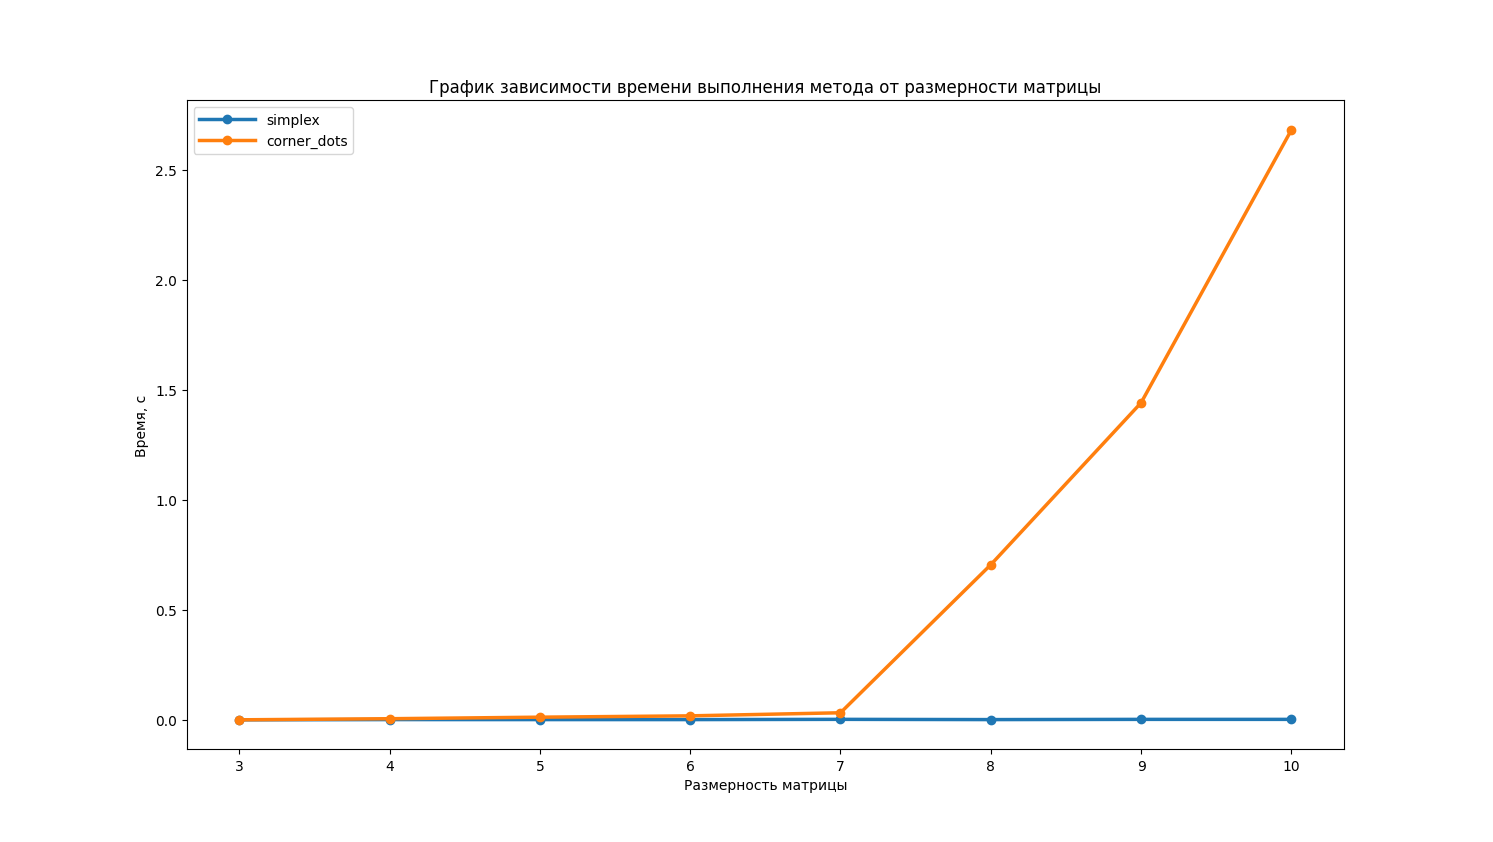
\includegraphics[width=\textwidth]{../graphics/time_3_11_1.png}
        \end{center}
        Для матриц маленького (<4) ранга Симплекс метод и метод перебора крайних точек,
	дают похожие результаты по времени. Что логично, ведь методу перебора крайних точек
	нужно перебрать не так много матриц (максимум 16). В дальнейшем количество матриц для перебора быстро увеличивается
	и метод перебора крайних точек начинает существенно проигрывать симплекс методу в таблицах.
	Отрыв, хорошо видно на "графике 2".


        \item График зависимости времени выполнения Симплекс метода от размерности матрицы в среднем (10,50)
        \begin{center}
         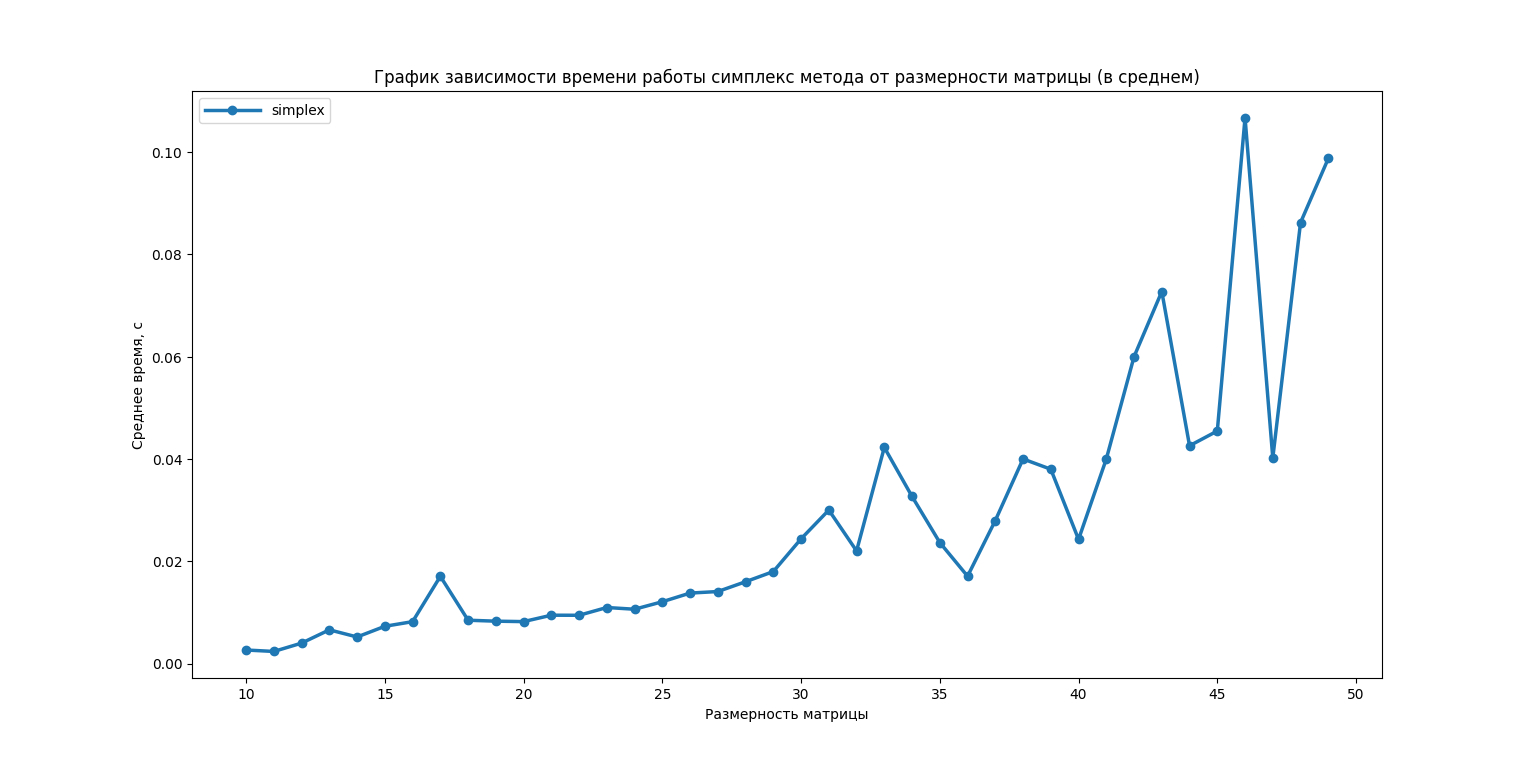
\includegraphics[width=\textwidth]{../graphics/simplex_time_rangs_many.png}
        \end{center}
        Был произведён замер времени (10 раз). И взято среднее значение. Видно, что с ростом размерности матрицы время работы Симплекс метода увеличивается (не монотонно).
Немонотонность обусловлена возможностью в некоторых тестовых запусках очень быстро получить целевую функцию, удовлетворяющую критериям остановки метода. (Все коэффициенты >0)
    \end{enumerate}

    \subsection{Теоретическая оценка алгоритмов}
    Инициализация Симплекс метода, зачастую более затратная чем реализация самого Симплекс метода (по времени и памяти)
т.к при инициализации добавляются дополнительные переменные (количество зависит от количества отрицательных компонент
вектора b) и приходится решать задачу более высокого порядка.

    Ищем выводимую строку и вводимый столбец $(O(n))$.
    Выполняем процедуру pivot (Жордано Гаусс) $(O(n^2))$
    Эти операции в худшем случае выполнятся $C^m_n$ раз. Где n - число столбцов, m - число строк.
    Можно сделать вывод , что в худшем случае симплекс метод работает за $O(2^n)$

    \section{Дополнительные исследования}

    Приведем соответствие Симплекс-Метода и Табличного Симплекс-Метода\\
    Каждому шагу Табличного Симплекс-Метода сопоставим шаг обычного Симплекс-Метода\\

    1.1) Предподготовка. Данная в общей форме задача приводится к каноническому виду. После этого выделяется первый базис. Причем коль скоро этот базис состоит из линейно независимых векторов, мы будем приводить эти вектора к единичному виду (м. Жордано-Гаусса). Таким образм подматрица $A[M, N_k]$ будет являтся матрицей перестановок. Никто не мешает представить вектор $c$ таким образом, чтобы он был выражен только через небазисные компоненты. Так и поступим. \\

    1.2) Все образования п.1.1 приводят к эквивалектной задача Л.П., поэтому на вход обоим Симплекс-Методам подается все та же исходная задача\\

    2.1) Проверка условий оптимальности. В Табличном Симплекс-Методе при решении задачи минимизации условием прекращения алгоритма является условие $c^T[L_k] \geq 0$ \\

    2.2)
    \begin{center}
        $y^T[M] = c^T[N_k] * B[N_k, M] = 0$ \\
         $c^T[L_k] - y^T[M] * A[M, L_k] \geq 0$ \\
         $c^T[L_k] \geq 0$
         $=>$ условия эквивалентны \\
    \end{center}


    3.1) Замена базиса. В задаче минимизации по заданному правилу выбирается вводимый столбец $j_k$ (среди отрицательных компонент вектора $c$ выбирается наибольший по модулю. Координата данного столбца - это номер вводимого столбца). Среди компонент выбранного столбца либо не существует положительных компонент, и тогда решения задачи не ограничено, либо существуют положительные компоненты. Тогда среди отношений $b[i]/ A[i, j_k]$ выбирается минимальное положительное (**). Базисная компонента, взятая по номеру найденного отношения  - выводимый столбец. Далее - процедура pivot (см. Корман) и обновление вектора $c$ по вышеуказанному правилу (эквивалентное преобразование). \\

    3.2) $j_k$ выбирается по тому же правилу. В обычном Симплекс - Методе:
    \begin{center}
        $x_{k+1}[N] = x_k[N] - \theta * u_k[N]$, где (*) \\
        $u_k[j_k] = -1$, \\
        $u_k[L_k \ j_k] = 0$\\
        $u_k[N_k] = B[N_k, M] * A[M, j_k]$
    \end{center}

        % Причем $B[N_k, M]$ - матрица перестановок (по построению). Из этого следует, что $u_k[N]$ состоит из перестановки вектора $A[M, j_k]$, нулей и одной (-1)\\
        $B[N_k, M]$ - матрица перестановок, поэтому $x_k[N]$ - вектор, состоящий из нулей и перестановки вектора $b$ (равенство "почти единичной" матрицы, умноженной на $x_k[N_k]$, вектору $b$).
        Поэтому правая часть (*) эквивалентна тому, что из вектора $x_k[N_k]$ мы вычитаем вектор $A[M, j_k]$ (дополненный нулями и минус единицей) с коэффиициентом $\theta$.\\
        $\theta$ подбирается таким образом, чтобы при вычитании обнулить выводимую переменную, при этом оставив базис допустимым и не переведя вдруг одну из компонент вектора $x[N_k]$ в отрицательную область. \\
        Выбор $\theta = min(x_k[i] / u_k[i]), u_k[i] > 0$ в обычном Симплекс-Методе соответствует решению (**) из п.3.1, потому что $x_k[N_k] = b[M]$ по построению, а $u_k[i] > 0$ только на коэфиициентах $A[M, j_k]$.\\
        Если не существует $u_k[i] > 0$, то задача не ограничена. Это соответствует аналогичному выводу табличного метода, поскольку в таком случае $A[M, j_k] \leq 0$, остальные же компоненты - это нули и минус единица.\\
        Процедура pivot обновляет вектор $b_k[M]$ таким образом, что $b_{k+1}[M] = b_k[M] - \theta * A[M, j_k]$, что эквивалентно (*). Вспомним, что по построению $x_k[N_k] = b[M]$. Это доказывает эквивалентность табличного и обычного Симплекс-Методов.


    \section{Выводы}
    В работе были проведены исследования по сравнению двух методов нахождения оптимального решения задачи линейного программирования. (Метод крайних точек и Симплекс метод)
Исходя из полученных результатов, можно сделать следующие выводы:
\begin{enumerate}
    \item Для матриц маленькой размерности ($\le 5$) оба метода дают решение за примерно одинаковое время.
    \item Для матриц большей размерности Симплекс метод существенно начинает выигрывать по скорости у метода перебора крайних точек . "Существенность" выигрыша растет при росте размерности матриц.
    \item Время работы Симплекс метода прямо пропорционально размерности матрицы. Выбросы обусловлены "случайностью" входных данных. (Можем очень быстро получить целевую функцию с положительными коэффициентами)
\end{enumerate}

	\section{Библиографический список}
	\begin{enumerate}
    \item Кормен, Томас Х., Лейзерсон, Чарльз И., Ривест, Рональд Л., Штайн, Клиффорд. "Алгоритмы. Построение и анализ, 2-е издание" Издательский дом “Вильямс”, 2011. -- 892--918 с.

    URL: \url{https://vk.com/doc191450968_561608466?hash=HUwStWS0yzrW9SaXn8POZtaz3gTyMTmLBxPGZpnqDrc&dl=U9ivclLJBeeYQbs3MMhGtwYZ7Mx4nGJelTv0Hv56E4z} / [Электронный ресурс]. Режим доступа:  (Дата обращения: 17.02.2023)

    \item Родионова Е.А., Петухов Л.В., Серёгин Г.А. "Методы оптимизации. Задачи выпуклого программирования" Издательство Политехнического университета, Санкт-Петербург, 2014

    URL: \url{https://elib.spbstu.ru/dl/2/i17-98.pdf/info} / [Электронный ресурс]. Режим доступа:  (Дата обращения: 20.02.2023)

    \item Моисеев Н.Н. "Методы оптимизации"

    URL: \url{https://avidreaders.ru/book/metody-optimizacii-1.html}/ [Электронный ресурс]. Режим доступа:  (Дата обращения: 22.02.2023)


	\end{enumerate}


\end{document}